\section{Results}
We employed RBR on a constructed gold standard where the exact displacement was known. By taking an undistorted FLASH image and realistically distorting the cortical surface by means of a field map, we could test if we could retrieve the initial position of the boundaries. In Fig~\ref{fig:registrationhistogram}, we present a histogram of the displaced boundaries and the registered boundaries, both with respect to the true position. The registered boundaries clearly show a sharp distribution centred around the origin ($\mu=0.027$ mm). The FWHM of the distribution is $0.49$ mm, showing that RBR provides accurate submillimetre registration. Additionally, Fig.~\ref{fig:flashregistration} shows a cross section (middle slice of the volume) of the registration.
\begin{figure}[!ht]
\centering
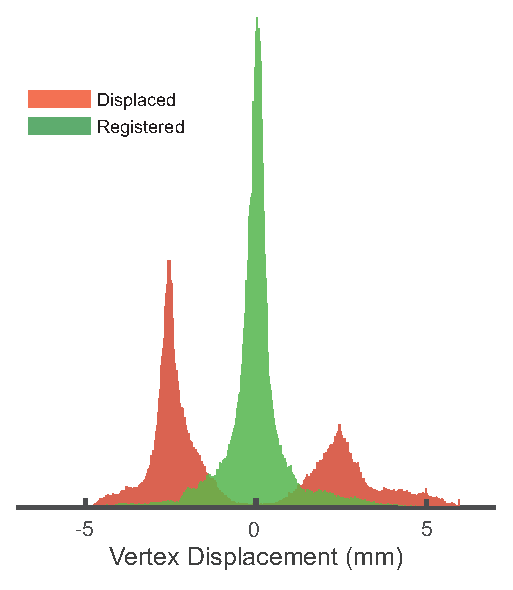
\includegraphics[width=0.4\textwidth, clip=true]{./Chapters/02_Registration/Images/./Histograms}
%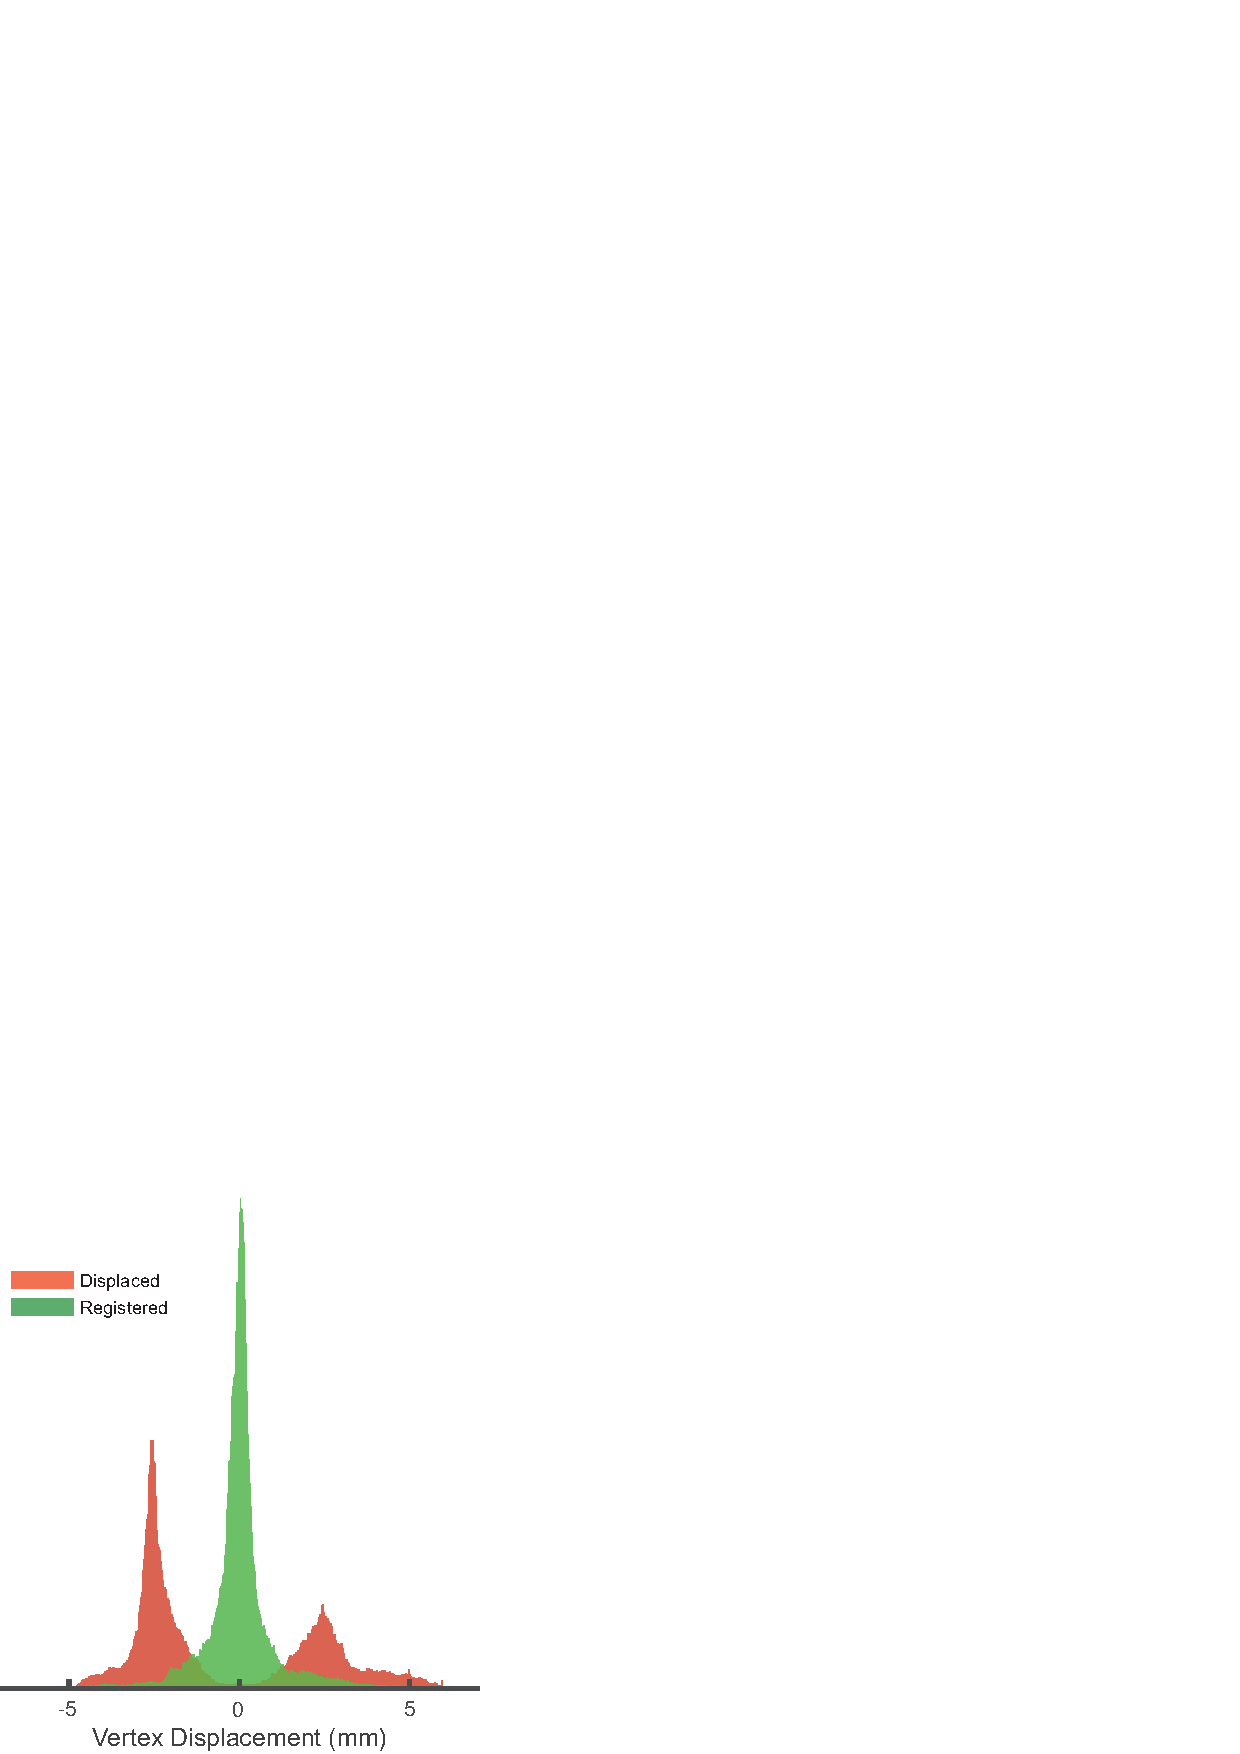
\includegraphics[width=0.4\textwidth, clip=true]{./Chapters/02_Registration/Images/./Images/Histograms.png}
\caption{Histogram of the displacement of all 228,208 vertices within a single brain mesh. The {\color{red}red} histogram shows the displacement after fieldmap based distortion with respect to a gold standard. The {\color{green}green} shows the displacement after applying RBR with respect to the same standard. After registration, the histogram clearly shows a sharp zero-centered (no bias) distribution.}
\label{fig:registrationhistogram}
\end{figure}
\begin{figure}[!ht]
\centering
\includegraphics[width=0.9\textwidth, clip=true]{./Chapters/02_Registration/Images/./FLASH_registration}
%\includegraphics[width=0.9\textwidth, clip=true]{./Chapters/02_Registration/Images/./Images/FLASH_registration.png}
\caption{The mid slice of the registration performed on a manually distorted FLASH image (red boundaries). The registered surface (yellow) overlaps for the larger part of the brain almost perfectly with the gold standard (green). If the specificity is set to high values, there is a risk that errors start to appear in some low contrast regions. This largely depends on the balance between false positives and false negatives in terms of corrected regions.}
\label{fig:flashregistration}
\end{figure}

In most of the slice (and the volume), the registration accuracy is well within the submillimetre regime. However, especially in low contrast areas the algorithm may show some small inaccuracies. This mainly proliferates when there is also another gradient in the image (e.g. the pial surface) on which the algorithm starts to fix the boundaries. This is largely related to the fine line between obtaining sufficient specificity and overfitting the data.

% % EPI
We performed RBR on a (resting state) dataset intended for laminar analysis consisting of 11 subjects. The boundaries after a 12 DoF \texttt{bbregister} were recursively registered to the mean EPI images (0.93 mm isotropic resolution) and this yielded an updated cortical surface. The new surface followed the grey matter boundary in the volume visibly better than the unregistered one. In Fig.~\ref{fig:epiregistration} we present a single slice with both sets of boundaries overlaid on top of them, illustrating the improvement. We here present the data for a representative subject, and identical images for all other subjects are presented in the Supplemental Materials.
\begin{figure}[!t]
\centering
\includegraphics[width=0.7\textwidth, clip=true]{./Chapters/02_Registration/Images/./EpiRegistration}
%\includegraphics[width=0.8\textwidth, clip=true]{./Chapters/02_Registration/Images/./Images/EpiRegistration.png}
\caption{
	Distortion correction of 7T 3D EPI data, obtained with 0.93 mm isotropic resolution. In {\color{red}red}, the original brain surfaces are shown after a 12 DoF registration performed by \texttt{bbregister}. The mesh in {\color{green}green} is the updated mesh by means of the first stage RBR, 2 DoF (scale and translation in the PE direction). The green boundaries follow the white matter boundary much better. The voxel displacement map (lower right) shows displacements on the order of several millimetres. The control point lattice that was used to displace the boundaries are overlaid onto the displacement map. Similar images for all subjects can be found in the supplementary materials. For even better inspection, movie files for all subjects are included in the online supplemental materials.} 
\label{fig:epiregistration}
\end{figure}

Additionally, Fig~\ref{fig:aad} shows the Absolute Average Displacement (AAD) of the registration on salted images with respect to the registration on the no-noise volume. Even for highly noisy images, the registration improves somewhat with respect to the undisplaced boundaries. In the absence of a gold standard model of the distortions, the monotonic decrease of the AAD indicates that RBR converges to an optimum as a function of data quality.
\begin{figure}[!ht]
\centering
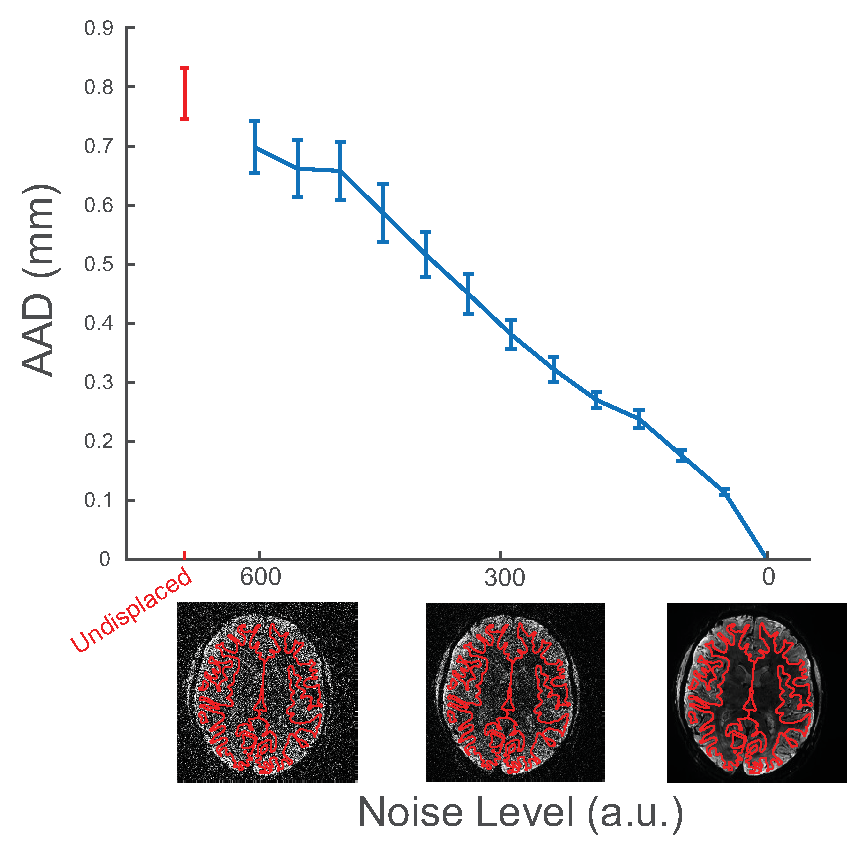
\includegraphics[width=0.7\textwidth, clip=true]{./Chapters/02_Registration/Images/./AAD}
%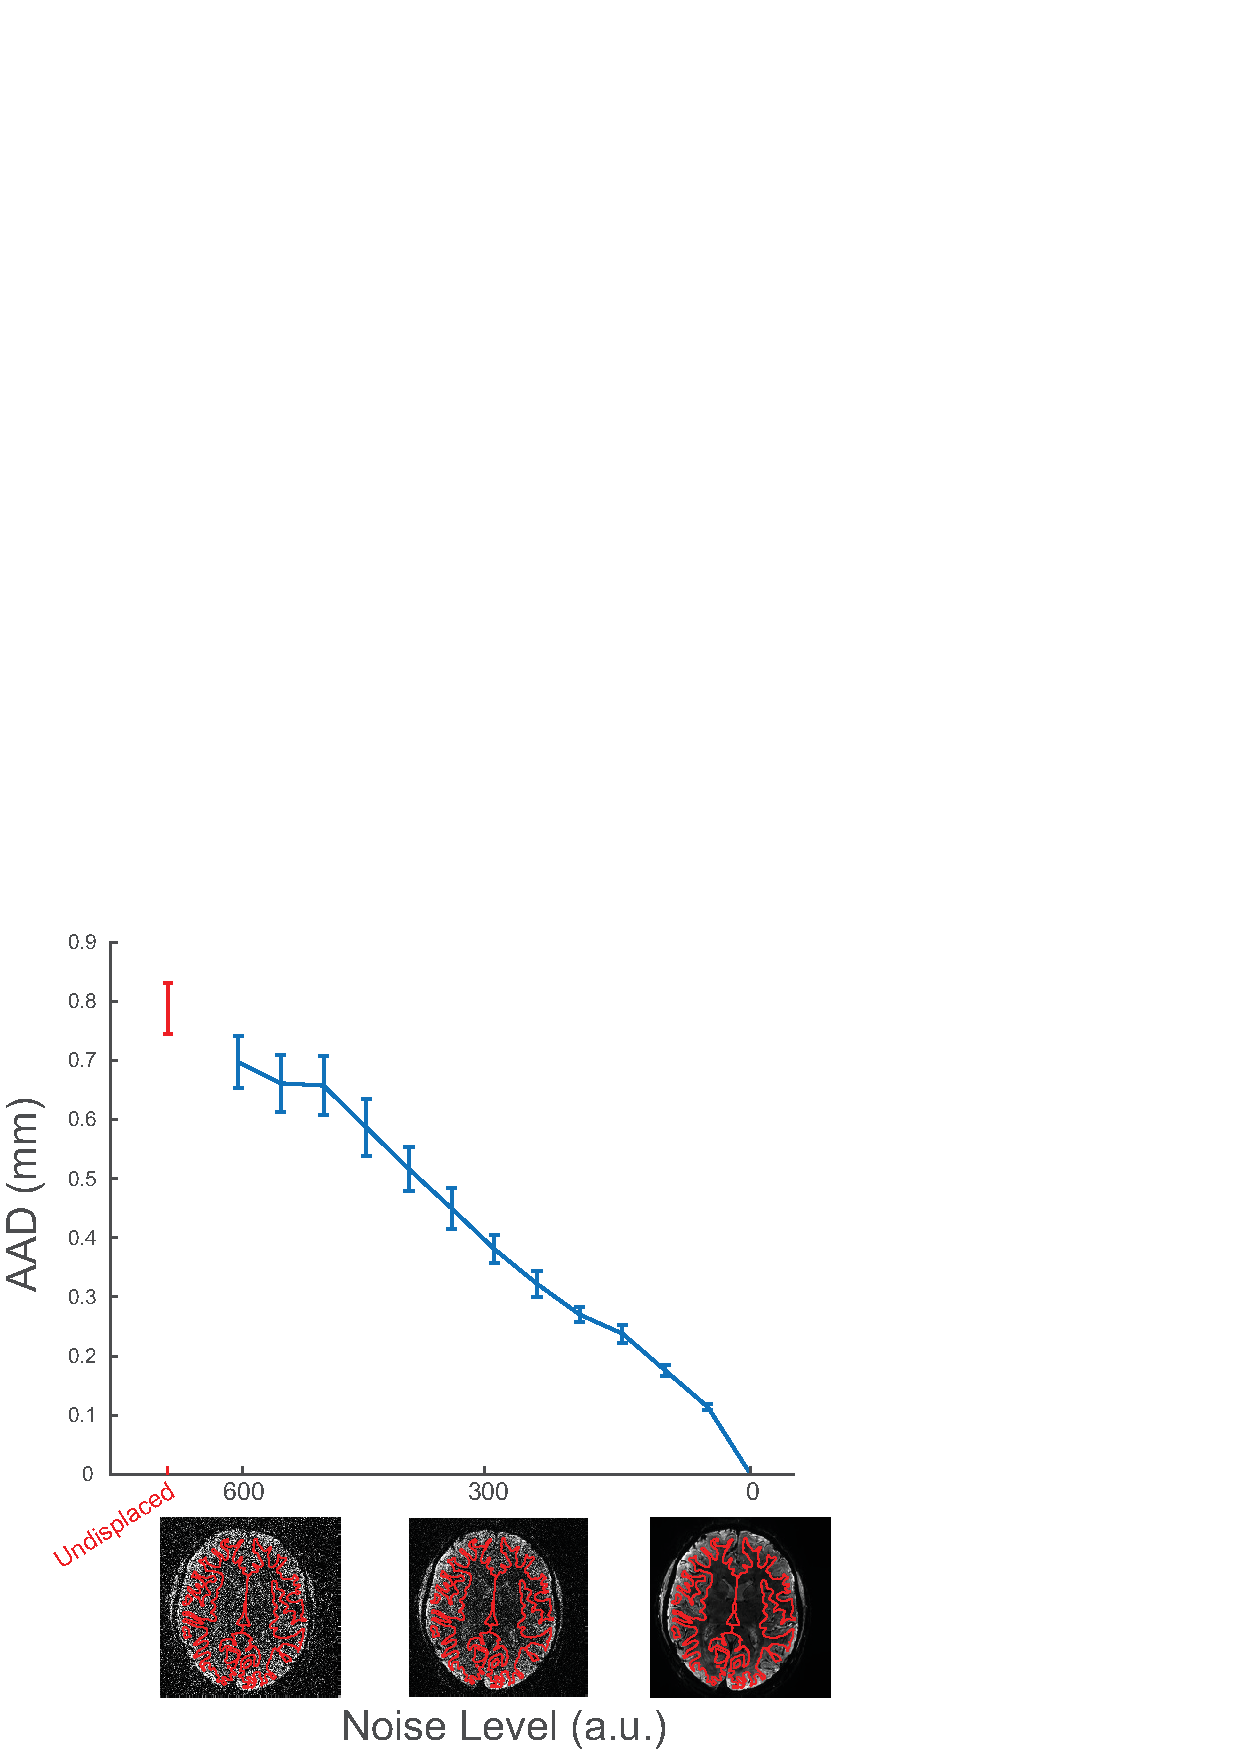
\includegraphics[width=0.7\textwidth, clip=true]{./Chapters/02_Registration/Images/./Images/AAD.png}
\caption{
	The effect of adding noise on the computed average absolute displacement with respect to a no-noise registration. In the absence of knowledge about the true distortions, the monotonic decrease of the AAD indicates that RBR converges to an optimum as a function of data quality.}
\label{fig:aad}
\end{figure}

\subsection{Data Availability}
All source code for the registration algorithm is freely available under the GPL 3.0 license at \url{https://github.com/TimVanMourik/OpenFmriAnalysis}. The respective modules are also available in Porcupine \url{https://timvanmourik.github.io/Porcupine}, a visual pipeline tool that automatically creates custom analysis scripts \cite{VanMourik2017}. All code to generate the images in this paper are available at the Donders Repository \url{https://data.donders.ru.nl/collections/shared/di.dccn.DSC_3015016.05_558/id/27015532}. This also includes additional movie files that scroll through the volumes, which is highly relevant to fully investigate whole brain registration performance. 
\begin{figure}[!ht]
\centering
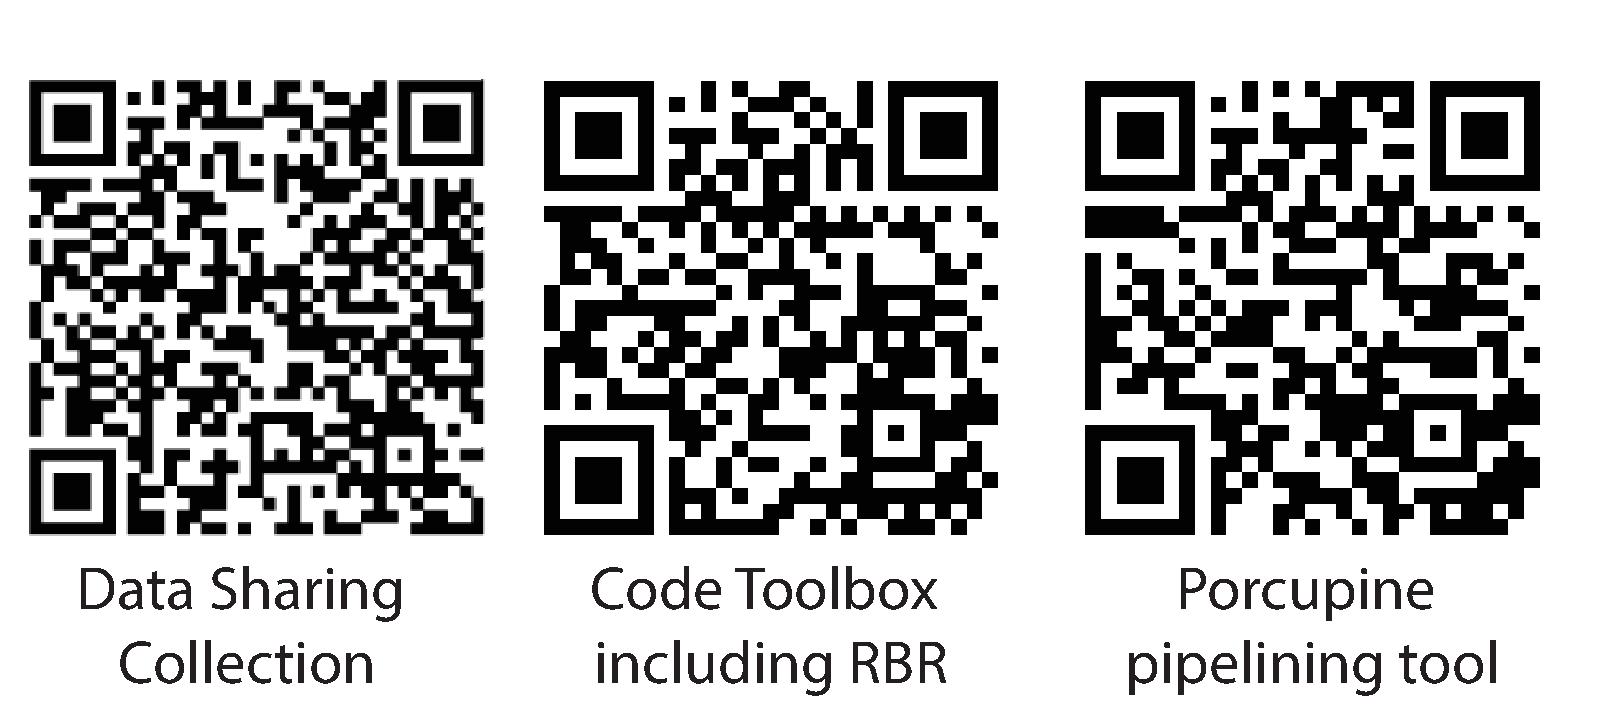
\includegraphics[width=0.3\textwidth, clip=true]{./Chapters/02_Registration/Images/./QRCodes}
%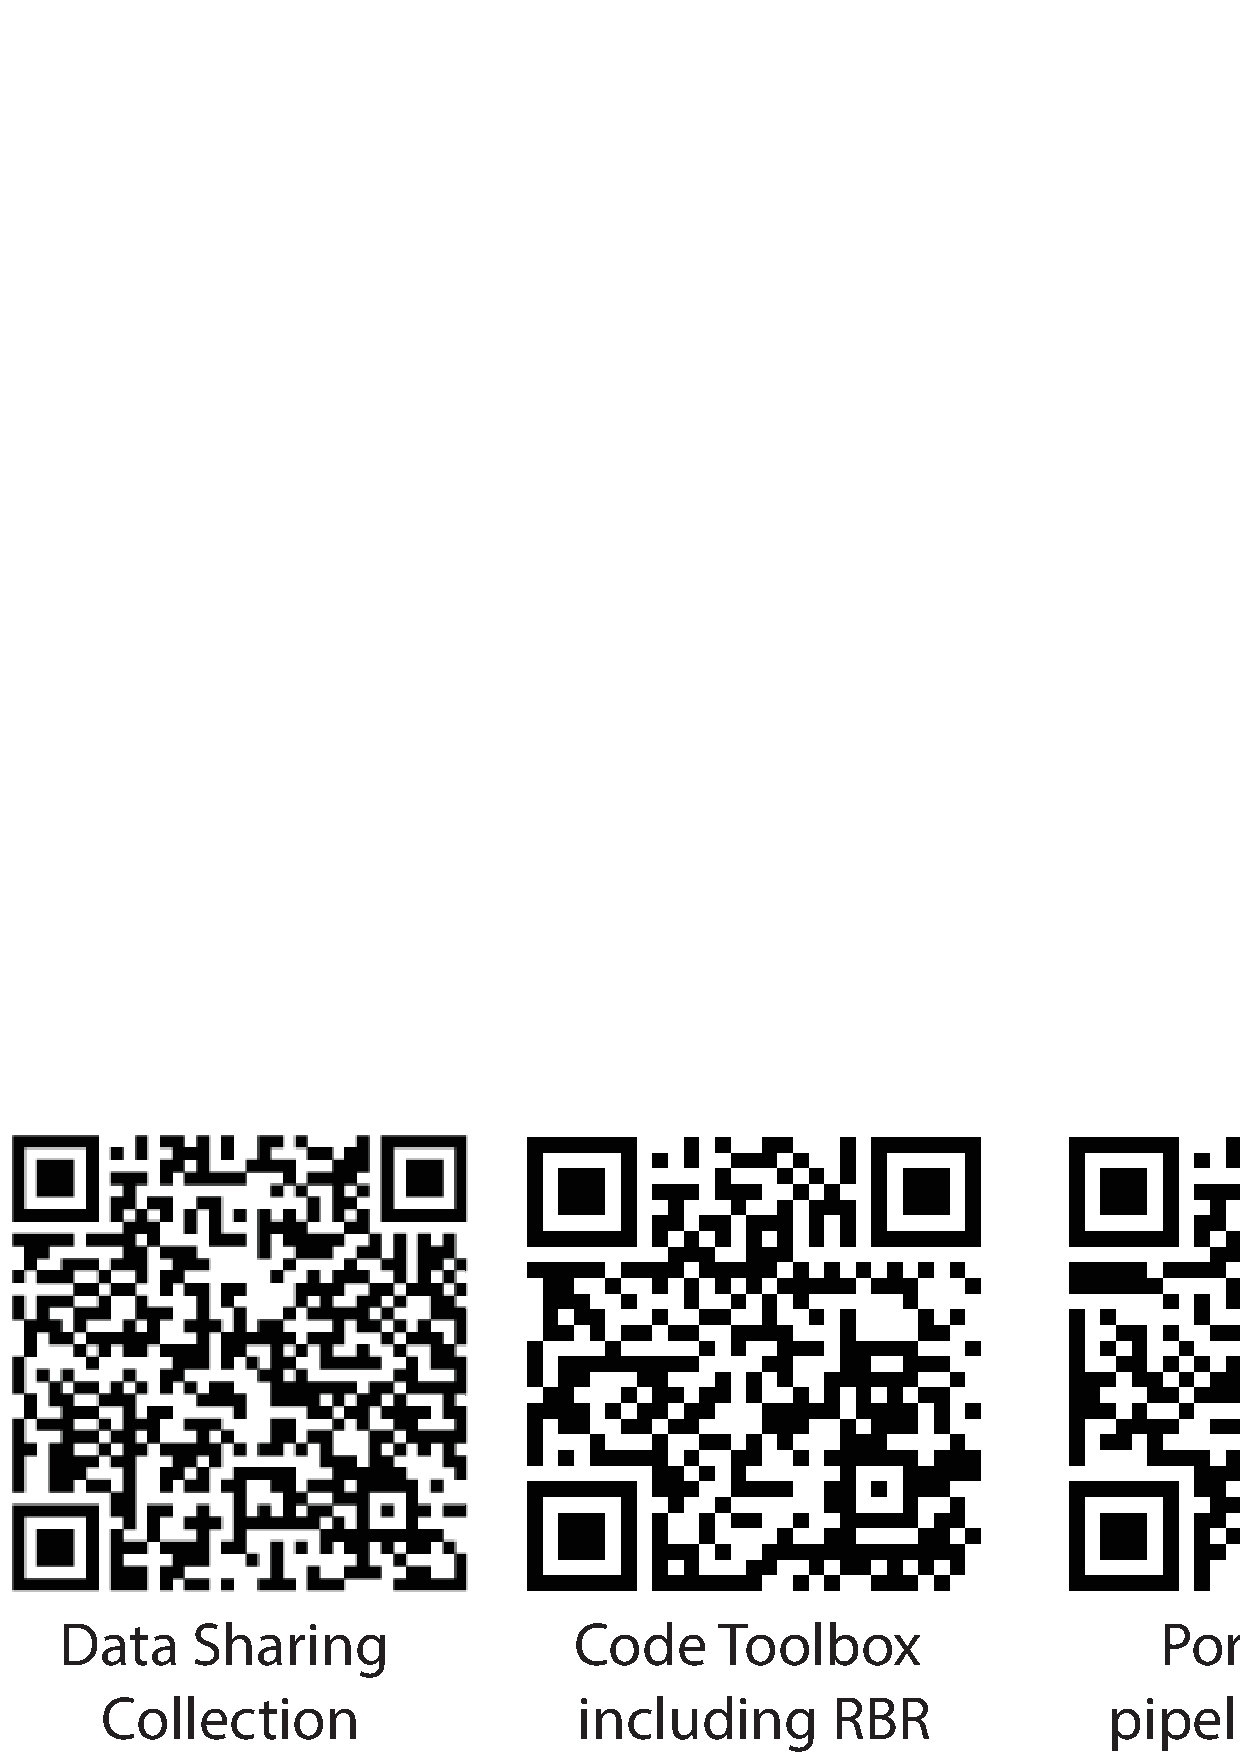
\includegraphics[width=0.5\textwidth, clip=true]{./Chapters/02_Registration/Images/./Images/QRCodes.png}
\caption{The links to, respectively, the source code of the algorithms, the analysis scripts for creating all figures in this paper, and the pipeline tool to easily incorporate it in one's custom analysis.}
\label{fig:si-qrcodes}
\end{figure}


